% Taken from:
% http://steventhornton.ca/blog/markov-chains-in-latex.html
\documentclass{standalone}
\usepackage{adjustbox}
\usepackage{tikz}
\usetikzlibrary{automata, positioning, backgrounds, calc, arrows}
\definecolor{light}{RGB}{188, 188, 220}
\definecolor{mid}{RGB}{124, 124, 185}
\definecolor{dark}{RGB}{39, 39, 143}
\definecolor{highlight}{RGB}{180, 31, 180}
\begin{document}
\begin{adjustbox}{max width=1.0\textwidth}
    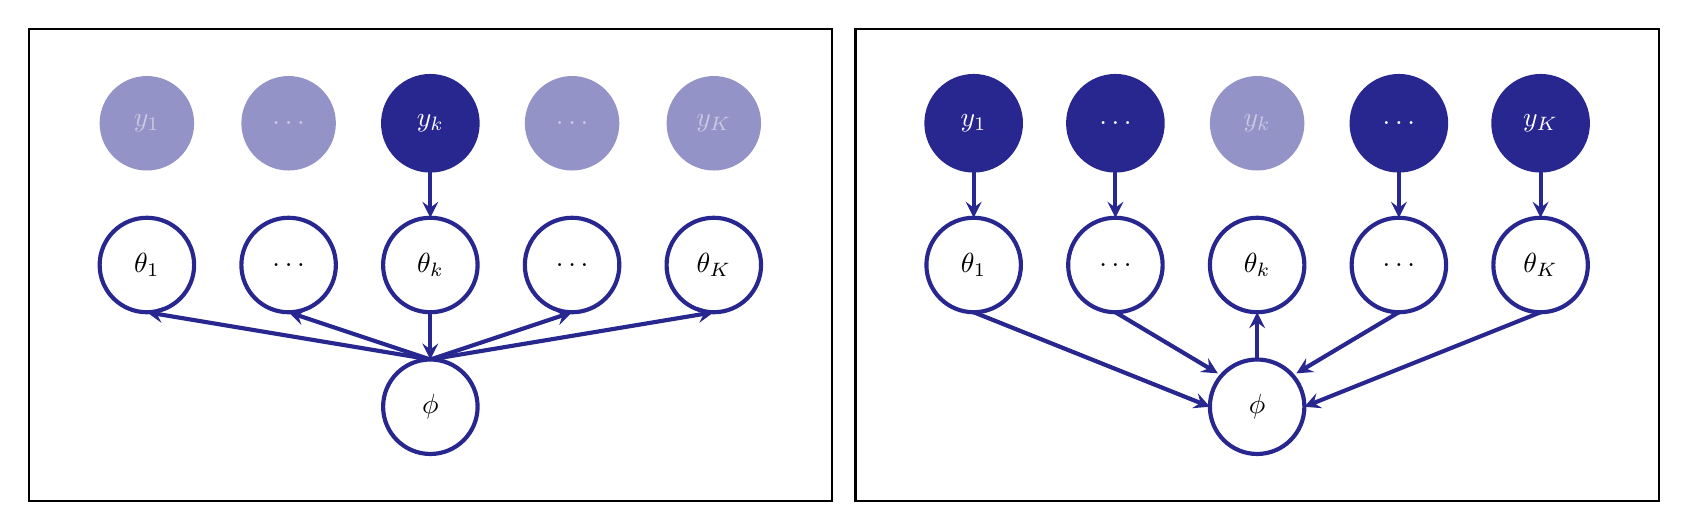
\begin{tikzpicture}[scale=0.3, thick]

        % Right
        \pgfmathsetmacro{\r}{2}

        \pgfmathsetmacro{\dx}{0}
        \pgfmathsetmacro{\dy}{0}

        \draw[black] (-17 + \dx, -7 + \dy) rectangle (17 + \dx, 13 + \dy);

        \fill[fill=dark, line width=1.5, opacity=0.50] (-12 + \dx, 9 + \dy) circle (\r)
        node[color=white] { $y_{1}$ };

        \fill[fill=dark, line width=1.5, opacity=0.50] (-6 + \dx, 9 + \dy) circle (\r)
        node[color=white] { $\ldots$ };

        \filldraw[fill=dark, draw=dark, line width=1.5] (0 + \dx, 9 + \dy) circle (\r)
        node[color=white] { $y_{k}$ };

        \fill[fill=dark, line width=1.5, opacity=0.50] (6 + \dx, 9 + \dy) circle (\r)
        node[color=white] { $\ldots$ };

        \fill[fill=dark, line width=1.5, opacity=0.50] (12 + \dx, 9 + \dy) circle (\r)
        node[color=white] { $y_{K}$ };

        \draw[<-, >=stealth, color=dark, line width=1.5] (0 + \dx, 3 + \r + \dy) -- (0 + \dx, 9 - \r + \dy);

        \filldraw[fill=white, draw=dark, line width=1.5] (-12 + \dx, 3 + \dy) circle (\r)
        node[color=black] { $\theta_{1}$ };

        \filldraw[fill=white, draw=dark, line width=1.5,] (-6 + \dx, 3 + \dy) circle (\r)
        node[color=black] { $\ldots$ };

        \filldraw[fill=white, draw=dark, line width=1.5] (0 + \dx, 3 + \dy) circle (\r)
        node[color=black] { $\theta_{k}$ };

        \filldraw[fill=white, draw=dark, line width=1.5] (6 + \dx, 3 + \dy) circle (\r)
        node[color=black] { $\ldots$ };

        \filldraw[fill=white, draw=dark, line width=1.5] (12 + \dx, 3 + \dy) circle (\r)
        node[color=black] { $\theta_{K}$ };

        \draw[->, >=stealth, color=dark, line width=1.5] (0 + \dx, -3 + \r + \dy) -- (-12 + \dx, 3 - \r + \dy);
        \draw[->, >=stealth, color=dark, line width=1.5] (0 + \dx, -3 + \r + \dy) -- (-6 + \dx, 3 - \r + \dy);
        \draw[<-, >=stealth, color=dark, line width=1.5] (0 + \dx, -3 + \r + \dy) -- (0 + \dx, 3 - \r + \dy);
        \draw[->, >=stealth, color=dark, line width=1.5] (0 + \dx, -3 + \r + \dy) -- (6 + \dx, 3 - \r + \dy);
        \draw[->, >=stealth, color=dark, line width=1.5] (0 + \dx, -3 + \r + \dy) -- (12 + \dx, 3 - \r + \dy);

        \filldraw[fill=white, draw=dark, line width=1.5] (0 + \dx, -3 + \dy) circle (\r)
        node[color=black] { $\phi$ };

        % Left
        \pgfmathsetmacro{\dx}{35}
        \pgfmathsetmacro{\dy}{0}

        \draw[black] (-17 + \dx, -7 + \dy) rectangle (17 + \dx, 13 + \dy);

        \filldraw[fill=dark,  draw=dark, line width=1.5] (-12 + \dx, 9 + \dy) circle (\r)
        node[color=white] { $y_{1}$ };

        \filldraw[fill=dark,  draw=dark, line width=1.5] (-6 + \dx, 9 + \dy) circle (\r)
        node[color=white] { $\ldots$ };

        \fill[fill=dark, line width=1.5, opacity=0.50] (0 + \dx, 9 + \dy) circle (\r)
        node[color=white] { $y_{k}$ };

        \filldraw[fill=dark, draw=dark, line width=1.5] (6 + \dx, 9 + \dy) circle (\r)
        node[color=white] { $\ldots$ };

        \filldraw[fill=dark, draw=dark, line width=1.5] (12 + \dx, 9 + \dy) circle (\r)
        node[color=white] { $y_{K}$ };

        \draw[<-, >=stealth, color=dark, line width=1.5] (-12 + \dx, 3 + \r + \dy) -- (-12 + \dx, 9 - \r + \dy);
        \draw[<-, >=stealth, color=dark, line width=1.5] (-6 + \dx, 3 + \r + \dy) -- (-6 + \dx, 9 - \r + \dy);
        \draw[<-, >=stealth, color=dark, line width=1.5] (6 + \dx, 3 + \r + \dy) -- (6 + \dx, 9 - \r + \dy);
        \draw[<-, >=stealth, color=dark, line width=1.5] (12 + \dx, 3 + \r + \dy) -- (12 + \dx, 9 - \r + \dy);

        \filldraw[fill=white, draw=dark, line width=1.5] (-12 + \dx, 3 + \dy) circle (\r)
        node[color=black] { $\theta_{1}$ };

        \filldraw[fill=white, draw=dark, line width=1.5,] (-6 + \dx, 3 + \dy) circle (\r)
        node[color=black] { $\ldots$ };

        \filldraw[fill=white, draw=dark, line width=1.5] (0 + \dx, 3 + \dy) circle (\r)
        node[color=black] { $\theta_{k}$ };

        \filldraw[fill=white, draw=dark, line width=1.5] (6 + \dx, 3 + \dy) circle (\r)
        node[color=black] { $\ldots$ };

        \filldraw[fill=white, draw=dark, line width=1.5] (12 + \dx, 3 + \dy) circle (\r)
        node[color=black] { $\theta_{K}$ };

        \draw[<-, >=stealth, color=dark, line width=1.5] (-\r + \dx, -3 + \dy) -- (-12 + \dx, 3 - \r + \dy);
        \draw[<-, >=stealth, color=dark, line width=1.5] ({-0.25 - \r * cos(45) + \dx}, {-3 + \r * cos(45) + \dy}) -- (-6 + \dx, 3 - \r + \dy);
        \draw[->, >=stealth, color=dark, line width=1.5] (0 + \dx, -3 + \r + \dy) -- (0 + \dx, 3 - \r + \dy);
        \draw[<-, >=stealth, color=dark, line width=1.5] ({0.25 + \r * cos(45) + \dx}, {-3 + \r * cos(45) + \dy}) -- (6 + \dx, 3 - \r + \dy);
        \draw[<-, >=stealth, color=dark, line width=1.5] (\r + \dx, -3 + \dy) -- (12 + \dx, 3 - \r + \dy);

        \filldraw[fill=white, draw=dark, line width=1.5] (0 + \dx, -3 + \dy) circle (\r)
        node[color=black] { $\phi$ };
        \end{tikzpicture}
        \end{adjustbox}
\end{document}
